% Sollte größter Teil werden
% - High level overview?
% - Wie läuft das auf meinem System?
% - Code Dokumentation / Entwicklerdokumentation

%%%%%%%%%%%%%%%%%%%%%%%%%%%%%%%%%%%%%%%%%%%%%%%%%%
% Abschnitt - Grober Überblick
%%%%%%%%%%%%%%%%%%%%%%%%%%%%%%%%%%%%%%%%%%%%%%%%%%

%%%%%%%%
% Low level
% was muss ich als entwickler wissen
% tiles, parallelisierung, structs/klassen, struktur des projekts

% Zuordnung klasse -> Dokumentation
% backend
%   *.main.cpp, init -> Niels DONE
%   include Ordner und CMake -> Niels DONE
%   balancer + tests -> Florian
%   mandelbrot -> Florian (außer MandelbrotSIMD -> Niels DONE)
%   actors
%      Worker -> Tobi
%      Host
%         websocket-funktionen -> Niels
%         Rest -> Tobi
%           + Parallelisierungskonzept (+ welche MPI Method, warum)
%   structs/Netzwerk -> Tobi/Niels/Florian
%   dev-environment (was ist docker und wie/warum) -> Max
% frontend
%    connection -> Niels
%    tileDisplay -> Max
%        TileDisplay.ts
%            Prinzip 
%            genauer Ablauf/Funktionen
%               + Shader
%        WorkerLayer.ts
%           + Gruppierung
%        MatrixView.ts + RegionOfInterest.ts
%        Project.ts
%    visualization -> Niels
%    misc -> Max

\section{Dokumentation der Implementierung}

\subsection{Implementierung des Backends}

Zur hardwarenahe Berechnung der Mandelbrotmenge wird ein sogenanntes Backend gestartet.
Das in C++ programmierte Teilprojekt nimmt Rechenaufträge von einem Nutzer durch ein Frontend entgegen (auch
ein solches wird bereitgestellt), zerlegt sie und verteilt sie per MPI auf dedizierte Rechenknoten.
Dazu besteht das Backend aus zwei ausführbaren Dateien, \verb|host| und \verb|worker|.

\subsubsection{Inkludierte Header und CMake Anweisungen}

Sämtliche Headerdateien sind ohne Untergruppierung im Ordner \verb|include| des Projektes abgelegt.

Sie werden zusammen mit den Header-Bibliotheken \verb|rapidjson| und \verb|websocketpp| sowie der vorkompilierten
Bibliothek \verb|boost_static| von CMake eingebunden um das Projekt zu builden.

Für einen erfolgreichen Build wird CMake einer Version von mindestens 3.7.0 und die C++11 Standarts vorrausgesetzt.
Ergebnis des Builds sind die ausführbaren Dateien \verb|host| und \verb|worker| welche die
beschriebenen Funktionen innerhalb des Backends umsetzen.

Eine detailliertere Beschreibung ist im Anhang zu finden.

\subsubsection{Mainfunktion und Initialisierung}

Zur Initialisierung der Prozesse muss zunächst die MPI-Umgebung aktiviert und abgerufen werden.
Dies geschieht für beide Programme gleich, über die Initialisierungsfunktion in \autoref{src:init.cpp}.
Sie erwartet lediglich eine Beschreibung des Prozesses für den Log und eine Initialisierungsfunktion,
die erst zurückkehrt, wenn das Programm abgeschlossen ist und MPI beendet werden soll.
Die Funktion muss als Parameter den Rang bzw. die Id des aktuellen MPI-Prozesses und die Anzahl der initialisierten
Prozesse entgegen nehmen.

\subsection{Host Funktionalitäten}\label{cls:Host}

\subsubsection{Websocketverbindung}

Direkt nach der Initialisierung des Host-Programms wird ein separater Thread gestartet, der über Websocket
Anfragen zur Berechnung einer Region entgegennimmt sowie ein Thread, der berechnete Regionen an den verbundenen Client übergibt.
%Die Methode \verb|Host::start_server| initialisiert dabei lediglich den Websocketserver.
Über den Typ des Servers wird eine Kompression versendeter Nachrichten über die im Standart akzeptierte Extension \enquote{perMessageDeflate} aktiviert.
Zudem wird der Websocketserver mit \verb|server.init_asio()| mit der Transport Policy "transport::asio"
konfiguriert, sodass Multithreadzugriff auf Sende- und Empfangsmethoden problemlos möglich ist \cite{websocketppManual}.

Der Server behandelt zu jedem Zeitpunkt maximal eine Verbindung und speichert lediglich die zuletzt geöffnete Verbindung.

Empfangene Nachrichten werden mit der Methode \hyperref[cls:Host::handle_region_request]{\texttt{Host::handle\_region\_request}} behandelt.

Der zweite bei der Initialisierung gestartete Thread führt die Methode \hyperref[cls:Host::send]{\texttt{Host::send}} aus.

\paragraph{Host::handle\_region\_request}\label{cls:Host::handle_region_request}

Die Methode dekodiert einen empfangene Nachricht als JSON Regionsanfrage und behandelt sie nach folgendem Schema:

\begin{enumerate}
	\item Parse das empfangene RegionRequest-Objekt. Bei Fehlern wird die Funktion abgebrochen.
	\item Involviere den spezifizierten Lastbalancierer um eine Aufteilung der Region zu erhalten
	\item Bestimme den Rang des Workers, der eine Region bearbeiten wird. Hierzu wird der Algorithmus aus \autoref{src:Host.cpp.handle_region_request} verwendet.
	\item Sende die Aufteilung inklusive der Ränge aller beteiligten Worker als Regions-Objekt an das Frontend
	\item Übergebe die aufgeteilten Regionen an den Thread, der diese per MPI an die Worker sendet.
\end{enumerate}

In dem JSON wird unter dem Schlüssel \texttt{"balancer"} ein String erwartet, der den zu wählenden Lastbalancierer bestimmt.
Mögliche Zeichenketten hierfür sind in den Klassen der Balancierer unter \verb|backend/src/balancer| in der globalen Variable
\verb|Klassenname::NAME| gespeichert.

Es ist hierbei wichtig, dass das senden an die Worker erst nach der Antwort an das Frontend geschieht und wird daher garantiert.
Dadurch kann im Frontend sichergestellt sein, dass alle eintreffenden RegionData-Objekte zu einer Regionsaufteilung gehören,
die bereits empfangen wurde.

\paragraph{Host::send}\label{cls:Host::send}

Während ein Thread das Empfangen von Nachrichten übernimmt, behandelt diese Methode von den Workern fertig berechnete Regionen.
Die Methode setzt dabei eine Dauerschleife nach folgendem Schema um:

\begin{enumerate}
    \item Überprüfe auf das Vorhandensein fertig berechneter Regionen \label{enum:Host::send.step1}
    \item Ist keine Region verfügbar
    \begin{enumerate}
        \item Warte blockierend auf eine Änderung
        \item Springe zu Schritt \ref{enum:Host::send.step1}
    \end{enumerate}
    \item Ist eine Region verfügbar
    \begin{enumerate}
        \item Locke die geteilte Datenstruktur
        \item Entnimm eine Region daraus
        \item Löse das Lock
    \end{enumerate}
    \item Codiere die Regionsdaten in JSON und versende sie über Websocket an den aktuell verbundenen Client
    \item Springe anschließend zu Schritt \ref{enum:Host::send.step1}
\end{enumerate}

Ein Beispiel für versendete Regionsdaten kann \autoref{src:regionData.json} entnommen werden.

Mithilfe einer \texttt{condition\_variable}\footnote{\url{https://en.cppreference.com/w/cpp/thread/condition_variable}}
nutzt sie die C++11 nativen mutex-Mechanismen um über das Vorhandensein neuer Regionen informiert zu werden.

\subsection{Implementierung der Lastbalancierung}\label{sec:load_balancing}
Der Implementierung der Lastbalancierung liegen die in \autoref{sec:load_balancing_concepts} beschriebenen Konzepte zugrunde.
Wichtig bei der Umsetzung dieser ist, dass der garantierte Teiler (\verb|guaranteedDivisor|) von Höhe und Breite der Teilregionen dem der angeforderten Region entspricht (vgl. \autoref{fig:concept_coordinates}).
Eine Tile (ein Bereich mit Breite und Höhe gleich dem garantierte Teiler\footnote{Eine Region lässt sich also immer in eine ganzzahlige Anzahl von Tiles aufteilen, vgl. \autoref{fig:leafletTiles}}, die Bezeichnung \textit{Tile} kommt aus dem Frontend) muss also als atomare Einheit betrachtet werden, da es sonst im Frontend zu Schwierigkeiten bei der Darstellung kommt.

Die Klassenstruktur der Lastbalancierer entspricht dem Strategy-Pattern (vgl. \cite{gamma_design_1995} S. 315-323). So kann der Balancierer zur Laufzeit leicht gewechselt werden und auch die Erweiterung des Projekts um eine weitere Strategie gestaltet sich einfach.
Was dabei genau beachtet werden muss findet sich im Teil Erweiterung (\ref{lastbalancierung_erweiterung}).

\subsubsection{Naive Strategie}

Die naive Strategie (\verb|NaiveBalancer| und \verb|RecursiveNaiveBalancer|) lässt sich in beiden Varianten recht einfach nach dem oben beschriebenen Konzept umsetzen.
Zusätzlich wurde noch \verb|ColumnBalancer| implementiert, dabei handelt es sich um eine Variante des nicht-rekursive Ansatzes, die nur Spalten erzeugt.
Die Erhaltung des garantierten Teilers wird dadurch erreicht, dass die Höhe und Breite der Teilregionen auf ein Vielfaches dieses Teilers gesetzt werden.
Diese können bei der nicht-rekursiven Variante vor der eigentlichen Aufteilung bestimmt werden.
Da sich $\frac{width}{guaranteedDivisor}$ nicht unbedingt durch die Anzahl an Workern teilen lässt, kann es sein, dass einige Teilregionen um \verb|guaranteedDivisor| Pixel breiter sind.
Selbiges gilt für die Höhe.

Bei der rekursiven Variante wird mithilfe folgender Kriterien entschieden, ob horizontal oder vertikal geteilt wird:

\begin{itemize}
	\item Region vertikal oder horizontal nicht mehr teilbar (d.h. \verb|width| bzw. \verb|height| $\leq$ \verb|guaranteedDivisor|): Teile in die andere Richtung.
	\item Region vertikal und horizontal unteilbar: Erzeuge eine leere Region für die zweite Hälfte.
	\item Sonst: Teile parallel zur kürzeren Seite. Dies gibt dem Lastbalancierer mehr Möglichkeiten die Trennlinie zwischen den Teilregionen zu setzen, was zu einer genaueren Teilung führt.
\end{itemize}

Die Teilung an sich funktioniert wie die nicht-rekursive Aufteilung auf zwei Worker.
Der Rekursionskontext (\verb|struct BalancingContext|) wurde extern definiert, da dieser für die Strategie mit Vorhersage wiederverwendet wird.

\subsubsection{Strategie mit Vorhersage}

Auch diese Strategie (\verb|PredictionBalancer| und \verb|RecursivePredictionBalancer|) folgt den oben beschriebenen Konzept. 
Allerdings wurde die Berechnung der Vorhersage in eine eigene Klasse ausgelagert, da die Berechnung der Vorhersage für die rekursive und die nicht-rekursive Variante gleich ist.
Die Struktur der Vorhersage sorgt auch dafür, dass der garantierte Teiler erhalten bleibt.
Für die Berechnung der Vorhersage ist es notwendig, dass bei der Erststellung eine Referenz auf ein \verb|Fractal|-Objekt (siehe \ref{sec:mandelbrot_calculation}) erhalten.

\paragraph*{Bestimmung der Vorhersage}
% predicter
Die Vorhersage (\verb|struct Prediction|) wird von der Klasse \verb|Predicter| angestellt.
Dazu wird die Region in einer sehr viel geringeren Auflösung berechnet.
Die benötigte Anzahl an Iterationen wird jeweils pro Tile abgespeichert.
So wird sichergestellt, dass der garantierte Teiler auch nach der Aufteilung noch gilt, da die Balancierer die Vorhersage Eintrag für Eintrag verarbeiten.
Die Genauigkeit der Vorhersage kann über das Attribut \verb|predictionAccuracy| gesteuert werden:
\begin{itemize}
	\item $predictionAccuracy > 0$: $(predictionAccuracy)^2$ Pixel werden pro Tile berechnet. Die Summe der Iterationen für die einzelnen Pixel ergibt die Vorhersage für die Tile.
	\item $predictionAccuracy < 0$: Für $(predictionAccuracy)^2$ Tiles wird ein Pixel in der Vorhersage berechnet. Es erhalten also mehrere Tiles diesselbe Vorhersage.
	\item $predictionAccuracy = 0$: Es wird keine Vorhersage angestellt.
\end{itemize}
Zusätzlich beinhaltet die Vorhersage die Summen der benötigten Iterationen pro Spalte und Zeile, sowie die Gesamtsumme.
So wird vermieden, dass diese während des Balancierens immer neu berechnet werden müssen.

\paragraph*{Nicht-rekursive Variante}\label{lastbalancierung_vorhersage}
% non-recursive prediction
Für die nicht-rekursive Aufteilung wird die Region erst in Spalten aufgeteilt und in einem zweiten Schritt wird dann die horizontale Unterteilung in Teilregionen vorgenommen.
Da die beiden Schritte analog zueinander sind wird hier nur das Aufteilen in Spalten anhand des Pseudocodes in \autoref{src:prediction_pseudo} beschrieben.

Die optimale Rechenlast pro Spalte (\verb|desiredN|) berechnet sich nach \autoref{equ:desiredN} wobei die Anzahl der Worker durch die Anzahl an Spalten ersetzt werden muss.
Als Abschätzung der Gesamtrechenlast wird die Gesamtsumme der Vorhersage verwendet.
Eine Spalte, die als leere Region beginnt, wird nun solange um eine Spalte von Tiles vergrößert bis die optimale Rechenlast erreicht oder überschritten wird.
Dazu müssen die Spaltensummen der Vorhersage aufaddiert werden.
Um Lücken auszuschließen werden die Grenzen der Spalten explizit aufeinander gesetzt, d.h. bei zwei benachbarten Teilregionen entspricht die obere Grenze der Einen der unteren Grenze der Anderen.
Damit es auch für die Aufteilung in Teilregionen eine Vorhersage gibt, wird eine Kopie der Vorhersage erstellt, welche nur die Werte für die aktuelle Spalte enthält (nicht im PSeudocode).

\begin{figure}[!h]
	\begin{lstlisting}[language=python, caption={Aufteilung in Spalten im Pseudocode}, label={src:prediction_pseudo}]
		def balanceLoad (region, nodeCount)
			# Will be per tile
			prediction = sampleFractal(region)
			cols = computeColCount(nodeCount)
			deltaRes = region.guaranteedDivisor
			deltaReal = deltaReal(region)
			desiredN = computeOptimalLoad(prediction, cols)
			cur = region
			curN = 0
			colsMade = 0
			for i = 0 to prediction.cols.vectorLength
				if colsMade + 1 == cols
					cur = rest of region # Part of region thats not already assigned to a col
					result.append(cur)
					break
				curN += prediction.cols[i]
				cur.width += deltaRes
				cur.maxReal += deltaReal
				# Make sure that each col has at least width = deltaRes
				if curN >= desiredN OR prediction.cols.length - i - 1 < cols
					result.append(cur) # Copy of cur
					cur.minReal = cur.maxReal
					cur.width = 0
					curN = 0
					colsMade++
					continue
			return splitColsInParts(result)
	\end{lstlisting}
\end{figure}

Im eigentlichen Code wurden ein paar Optimierungen am Pseudocode vorgenommen.
Um float-Ungenauigkeitenbeim wiederholten Addieren zu minimieren werden die Werte in \verb|cur| nicht aufaddiert, sondern aus den Zählern berechnet.
Außerdem werden die Spalten ohne Zwischenspeicherung in die nötigen Teilregionen aufgeteilt.
Zusätzlich wird \verb|desiredN| nach jeder abgeschlossenen Spalte für die Verbleibenden neu berechnet, da es sehr unwahrscheinlich ist, dass dieser Wert genau erreicht wird.

\paragraph*{Rekursive Variante}
% recursive prediction
Die rekursive Variante der Strategie mit Vorhersage verwendet dasselbe Rekursionsschema wie ihr naives Gegenstück.
Also wird auch die Entscheidung, ob horizontal oder vertikal geteilt werden soll, auf die gleiche Art und Weise gefällt.
Der Unterschied zwischen den beiden Strategien liegt also hauptsächlich in den beiden Methoden zur Aufteilung.

Bei dieser Strategie werden die Regionen nicht einfach halbiert, sondern in zwei Teile aufgeteilt, die laut der Vorhersage ähnlich rechenintensiv sind.
Dazu wird ähnlich vorgegangen, wie bei der \hyperref[lastbalancierung_vorhersage]{nicht-rekursiven Variante} für die Aufteilung auf zwei Worker.
Deshalb profitiert diese Strategie auch besonders davon, dass immer parallel zur kürzeren Seite geteilt wird.
Die Vorhersage ist in diese Richtung nämlich feingliedriger, da weniger Tiles der Vorhersage zu einer Spalte bzw. Zeile zusammengefasst werden müssen als wenn parallel zur längeren Seite aufgeteilt werden würde.
Allerdings wird hier, wenn möglich, sichergestellt, dass beide Teilregionen groß genug sind um jeweils auf die Hälfte der Worker aufgeteilt zu werden.
Es ist hierbei auch wichtig die Vorhersage so zu teilen, dass es für jede Hälfte eine Vorhersage gibt, die dann an den rekursiven Aufruf übergeben werden kann.

\subsubsection{Erweiterung}\label{lastbalancierung_erweiterung}

Da die Lastbalancierung nach dem Strategy-Pattern realisiert ist, gestaltet sich die Erweiterung um eine neue Balancierungsstrategie recht einfach.
Zuerst muss eine Unterklasse von \verb|Balancer| (\autoref{src:Balancer.h}) erstellt werden, um ein gemeinsames Interface zu ezwingen und somit die polymorphe Nutzung der neuen Klasse zu ermöglichen.

\begin{figure}[h!]
	\lstinputlisting[caption={Das gemeinsame Interface der Lastbalancierung}, label={src:Balancer.h}, firstline=7, lastline=11]{../../backend/include/Balancer.h}
\end{figure}

Danach wird die neue Strategie über die Methode \verb|BalancerPolicy::chooseBalancer| verfügbar gemacht.
Dazu muss sie mithilfe der statischen Variablen \verb|Klassenname::NAME| benannt werden.
\verb|BalancerPolicy| muss nun so erweitert werden, dass, bei Eingabe des vorher festgelegten Namens, ein neues Objekt der entsprechenden Klasse zurückgegeben wird.
In \verb|BalancerPolicy| kann auch die Genauigkeit der Vorhersage für die oben aufgeführten Strategien festgelegt werden.

\paragraph*{Bedingungen an Balancer::balanceLoad}
Bei der Eingabe von \verb|region| und \verb|nodeCount| erfüllt ein korrekter Rückgabewert \verb|subregions| die folgenden Bedingungen:
\begin{itemize}
	\item \verb|subregions| ist ein Zeiger auf ein Array mit \verb|nodeCount| Elementen vom Typ Region
	\item Die Regionen in \verb|subregions| sind eine Partitionierung von \verb|region|, d.h. sie überschneiden sich nicht und ihre Vereinigung ergibt genau \verb|region|
	\item Für jede Region \verb|subregion| in \verb|subregions| gilt:
	      \begin{itemize}
		      \item \verb|guaranteedDivisor|, \verb|validation|, \verb|maxIteration| und \verb|fractal| sind in \verb|region| und \verb|subregion| gleich
		      \item \verb|subregion.guaranteedDivisor| teilt \verb|subregion.width| und \\ \verb|subregion.height| ohne Rest
		      \item \verb|subregion.hOffset| und \verb|subregion.vOffset| sind so gesetzt, dass sie den Abstand der oberen linken Ecke von \verb|subregion| zur oberen linken Ecke von \verb|region| in Pixeln angeben
		      \item Die Deltas für die komplexen Werte sind unverändert, d.h. die Größe des Bereiches der komplexen Ebene, der von einem Pixel abgedeckt wird, ist unverändert
		            % $\frac{region.maxReal - region.minReal}{region.width} = \frac{subregion.maxReal - subregion.minReal}{subregion.width}$ und \\ $\frac{region.maxImaginary - region.minImaginary}{region.height} = \frac{subregion.maxImaginary - subregion.minImaginary}{subregion.height}$
	      \end{itemize}
\end{itemize}

Ob diese Bedingungen erfüllt sind kann mit dem Test in \verb|BalancerTest| überprüft werden.
Dazu muss der neue Testfall (\verb|struct TestCase|) durch Angabe von Name, Anzahl an Workern, Balancierungsstrategie und Testregion spezifiziert werden.
Dann kann er an der im Quellcode markierten Stelle zum Vektor der Testfälle hinzugefügt werden.
Anschließend muss der Test mittels \verb|cmake| in \verb|backend/tests| neu kompiliert werden.

\subsection{Kommunikation der Prozesse per MPI}\label{sec:mpi}

% TODO: Irgendwo muss noch erwähnt werden, dass es nur auf gleichen Rechnern funktioniert, da wir Byte-Ströme übertragen

Das Message Passing Interface (MPI) wird ausschließlich im Backend zur Kommunikation zwischen dem Host und den Workern verwendet.

\paragraph{MPI und Threads}

Da sowohl im Host, als auch in den Workern mehrere Threads arbeiten, muss die Kompatibilität von MPI mit Threads genau betrachtet werden.
Laut der offiziellen \verb|MPI Dokumentation|\footnote{\url{https://www.mpi-forum.org/docs/mpi-3.1/mpi31-report.pdf}} müssen die konkreten Implementierungen von MPI keinerlei Threads unterstützen, die meisten bekannten Implementierungen (wie beispielsweise \verb|Open MPI|\footnote{\url{https://www.open-mpi.org/doc/v3.1/man3/MPI_Init_thread.3.php}}) tun dies aber, falls sie entsprechend konfiguriert wurden.

Es wurde besonders darauf geachtet, dass nur ein Thread pro Prozess MPI-Aufrufe tätigt, wodurch die Thread-Umgebung mit MPI\_THREAD\_FUNNELED initialisiert werden kann.
Dadurch kann MPI einige Optimierungen durchführen, die nicht möglich wären, wenn mehrere Threads MPI-Aufrufe tätigen.
Zudem sind die meisten MPI Implementierungen noch nicht auf eine performante Umsetzung von mehreren Threads ausgelegt, weshalb das Thread-Level so niedrig wie möglich gehalten werden sollte.

\paragraph{Busy-Waiting von MPI}\label{para:mpi_busy_waiting}

Bei den verwendeten Implementierungen von MPI, MPICH und OpenMP, wird bei blockierenden Nachrichtensende und -empfangsoperationen Busy-Waiting umgesetzt.
Das führt einerseits dazu, dass die Verzögerung beim Empfangen von Nachrichten minimiert wird und die Bearbeitung der Daten sofort starten kann.
Andererseits führt das aber zu einer 100-Prozentigen Auslastung des Rechenkerns, was andere Prozesse von der Durchführung ihrer Arbeit abhalten kann und zu einem erhöhten Stromverbrauch führt.

Im Fall des blockierenden MPI\_Recv wird solange aktiv ohne Pause getestet, ob eine Nachricht empfangen werden kann, bis dies der Fall ist.
Falls eine nicht-blockierende Empfangsoperation mit MPI\_Irecv gestartet wird, muss diese anschließend auch abgeschlossen werden.
Dazu kann einerseits MPI\_Wait dienen, das solange wartet, bis die Empfangsoperation abgeschlossen ist. Hierzu wird ebenfalls Busy-Waiting nutzt.
Andererseits kann auch MPI\_Test genutzt werden, was nur überprüft, ob die Empfangsoperation abgeschlossen ist ohne auf deren Abschluss zu warten.
Auch hier gibt es keine andere Möglichkeit, als immer wieder (beispielsweise in einer Schleife) MPI\_Test aufzurufen.
Der einzige Vorteil besteht darin, dass zwischen diesen wiederholten Aufrufen andere Arbeit erledigt oder der Prozess für eine gewisse Zeit schlafen gelegt werden kann.
Mit MPI\_Probe bzw. MPI\_Iprobe verhält es sich ähnlich wie mit MPI\_Recv bzw. MPI\_Test.
Also wird auch hier Busy-Waiting eingesetzt.

%TODO: x und y bestimmen. x=1?
In der Implementierung wurde deshalb im Host und im Worker ein eine nicht-blockierende Empfangsmethode gewählt, die den Thread für x Millisekunden schlafen legt, bevor Überprüft wird, ob Daten empfangen wurden.
Die damit einhergehende Verzögerung verfälscht das Ergebnis nicht schwerwiegend, da die Berechnung einer Region für gewöhnlich deutlich länger als y Millisekunden benötigt.
%TODO: Im Host das auch wirklich implementieren

\subsubsection{Genereller Aufbau der MPI-Kommunikation}

Im Folgenden wird kurz der generelle Aufbau der MPI-Kommunikationsroutinen im Host und in den Workern erklärt.

\paragraph{MPI-Kommunikation im Host}\label{para:mpi_generell_host}

%TODO: Evtl. Websocket-Thread erwähnen zu Beginn bei den neuen Aufträgen
Die essenziellen Teile der MPI-Kommunikation des Hosts, also das \hyperref[para:send_host]{Senden von Rechenaufträgen} und das \hyperref[para:recv_host]{Empfangen der berechneten Daten}, befinden sich in einer gemeinsamen Endlosschleife.
\begin{enumerate}
    \item Ist das Flag gesetzt, dass neue Rechenaufträge an die Worker zu senden sind \label{enum:Host::mpi.step1}
    \begin{enumerate}
        \item Sende alle Aufträge per MPI an die jeweiligen Worker. Der Rang bestimmt sich aus dem Index in der Datenstruktur für die Rechenaufträge.
    \end{enumerate}
    \item Können berechnete Daten von einem der Worker empfangen werden
    \begin{enumerate}
        \item Formatiere die empfangenen Daten, um Metainformationen hinzuzufügen
        \item Locke die mit dem Websocket-Sende Thread geteilte Datenstruktur.
        \item Lege die Daten in die Datenstruktur
        \item Löse das Lock
    \end{enumerate}
    \item Wurde keine Operation durchgeführt, schlafe $z$ ms, um die Prozessorlast zu verringern
    \item Springe zu Schritt \ref{enum:Host::mpi.step1}
\end{enumerate}

Dabei wird immer zuerst überprüft, ob neue Rechenaufträge an die Worker zu senden sind.
Gegebenenfalls werden die Sendeoperationen durchgeführt.
Anschließend wird überprüft, ob berechnete Daten empfangen werden können.
Ist das der Fall, so wird die Empfangsoperation durchgeführt, die Daten reorganisiert und über eine gemeinsame Datenstruktur an einen Websocket-Thread weitergeleitet, der die Informationen an das Frontend reicht.
Nun wird die Schleife von neuem begonnen.
Es wird also sowohl für das überprüfen, ob neue Rechenaufträge vorhanden sind, als auch für das Empfangen der berechneten Daten \hyperref[para:mpi_busy_waiting]{Busy-Waiting} eingesetzt.

\paragraph{MPI-Kommunikation im Worker}\label{para:mpi_generell_worker}

Auch hier wird das \hyperref[para:recv_worker]{Empfangen der Rechenaufträge} und das \hyperref[para:send_worker]{Senden der berechneten Daten} in einer Endlosschleife bewerkstelligt.
Zu beginn wird so lange gewartet, bis ein neuer Rechenauftrag empfangen wurde.
Direkt im Anschluss wird die Berechnung der empfangenen Region gestartet, wobei während der Kalkulation auf neu ankommende Rechenaufträge gelauscht wird.
Ist ein neuer Auftrag zu empfangen, so wird die laufende Berechnung abgebrochen und die Schleife von vorne gestartet.
Falls die Berechnung nicht unterbrochen wurde, werden die Daten organisiert und an den Host geschickt.
Nun beginnt die Schleife von vorne.

Es ist auch hier zu erkennen, dass \hyperref[para:mpi_busy_waiting]{Busy-Waiting} für das Empfangen von neuen Rechenaufträgen eingesetzt wird.

\subsubsection{Übertragung neuer Rechenaufträge vom Host an die Worker}

Um neue Rechenaufträge an die Worker zu übertragen, werden im Host und in den Workern Persistent Communication Requests verwendet. Das hat den Vorteil, dass der Kommunikationsoverhead zwischen dem Prozess und dem Kommunikationscontroller reduziert wird. Die Nutzung dieser Persistent Communication Requests ist möglich, da immer die selbe Datenmenge an die selben Empfänger gesendet wird bzw. vom selben Absender (das ist hier der Host) empfangen wird.

Zur Übertragung der neuen Rechenaufträge wird das Region-Struct verwendet, welches bereits durch einen Websocket-Thread ausgefüllt wurde.

\paragraph{Initialisierung der Persistent Communication Requests}\label{para:persistent_init}

Um die Persistent Communication Requests nutzen zu können, müssen diese zunächst Initialisiert werden.

Im Host werden hierzu ein Array mit MPI\_Request, ein Array mit MPI\_Status und ein Array mit Region erstellt. So bekommt jeder Prozess seinen eigenen Request, Status und Puffer für die zu sendende Region. Der Index, an dem sich diese Objekte befinden ist immer der von MPI zugewiesene Rang des Prozesses.
Anschließend wird die eigentliche Initialisierung der Persistent Communication Requests durch einen Aufruf von MPI\_Send\_init für jeden Prozess durchgeführt, wobei als Tag der Kommunikation die Zahl 1 gewählt wurde. Als Kommunikationsmodus wird eine nicht-blockierende Standardsendeoperation gewählt. Durch diesen Kommunikationsmodus wird die Senden-Operation nur gestartet, d.h. der Aufruf kehrt unter Umständen zurück, bevor die Sendeoperation abgeschlossen ist. Dadurch wird ein paralleles, möglichst schnelles Senden aller Rechenaufträge gewährleistet. Mehr zur Durchführung des Sendens ist im \hyperref[para:send_host]{nächsten} Paragraphen zu finden.
Die genaue Implementierung der Initialisierung ist in \autoref{src:mpi_send_init_host} zu sehen.

% Code in Worker anpassen, so dass Request, Status und Region zusammen mit MPI_Recv_init stehen
Im Worker werden ebenfalls jeweils ein MPI\_Request, ein MPI\_Status und ein Region Objekt erstellt. Dann wird wieder der Persistent Communication Request durch einen Aufruf von MPI\_Recv\_init initialisiert, wobei der Tag wieder 1 und die Empfangsoperation nicht-blockierend ist. Der Einsatz der nicht-blockierenden Empfangsoperation stellt sicher, dass der Worker laufende Berechnungen bei Erhalt eines neuen Rechenauftrags abbricht und sofort mit der Berechnung der neuen Anfrage beginnt. Mehr hierzu im Paragraphen \hyperref[para:recv_worker]{Empfangen der Rechenaufträge im Worker}.
Die Implementierung ist in \autoref{src:mpi_recv_init_worker} zu sehen.

\begin{figure}[h!]
	\lstinputlisting[caption={Initialisierung des Persistent Communication Requests im Host}, label={src:mpi_send_init_host}, firstline=525, firstnumber=525, lastline=531]{../../backend/src/actors/Host.cpp}
\end{figure}

\begin{figure}[h!]
	\begin{lstlisting}[language=c++, caption={Initialisierung des Persistent Communication Requests im Worker}, label={src:mpi_recv_init_worker}, firstnumber=56]
	// Init persistent asynchronous receive
	Region newRegion;
	MPI_Request request;
	MPI_Recv_init(&newRegion, sizeof(Region), MPI_BYTE, host_rank, 1, MPI_COMM_WORLD, &request);
	\end{lstlisting}
\end{figure}

\paragraph{Senden der Rechenaufträge im Host}\label{para:send_host}

Im Host sind neue Rechenaufträge immer dann an die Worker zu übertragen, wenn das Flag mpi\_send\_regions vom entsprechenden Websocket-Thread gesetzt wurde. Hierbei wird Busy-Waiting eingesetzt, da das Empfangen von fertig berechnenden Regionen auch nur mit Busy-Waiting funktioniert und sich das Senden und Empfangen in der selben Schleife befindet. Mehr hierzu in Abschnitten \hyperref[para:mpi_busy_waiting]{Busy-Waiting} und \hyperref[para:mpi_generell_host]{Genereller Aufbau der MPI-Kommunikation im Host}.

Sind neue Rechenaufträge verfügbar, wird jede einzelne Region einem verfügbaren Worker zugeordnet, wobei jeder Worker maximal eine Region bekommt.
Hierzu wird die Region aus der gemeinsamen Datenstruktur websocket\_request\_to\_mpi in den Sendepuffer des Workers kopiert. Anschließend wird das nicht-blockierende stardard Senden mit MPI\_Start gestartet.
Die Zuordnung zwischen Rang des Workers und Index der Region wird dabei Deterministisch bestimmt so wie in \autoref{src:Host.cpp.handle_region_request}.

% TODO: Evtl. anmerken, warum nicht gleich der Websocket-Thread in den Sendepuffer kopiert. Grund: Klare Trennung der beiden Threads und vermeiden von unauthorisierten Zugriff auf den Sendepuffer, weil ein lock vergessen wurde zu setzen o.Ä.

Falls nicht genügend Rechenprozesse zur Verfügung stehen (es also mehr zu berechnende Regionen als Rechenprozesse gibt), wird nur ein Fehler ausgegeben, da dieser Fall in der aktuellen Version unmöglich ist. Die restlichen Regionen, denen noch kein Rechenprozess zugeteilt wurde, werden nicht berechnet.
% In einer erweiterten Version durchaus möglich, aber extrem unwahrscheinlich.

Um sicherzustellen, dass alle Sendeoperationen abgeschlossen sind, wird MPI\_Waitall eingesetzt, welches den Thread des Hosts so lange blockiert, bis die Daten aus allen Sendepuffern ausgelesen wurden. Es wird jedoch nicht gewartet, bis das entsprechende Empfangen in den Workern gestartet bzw. beendet wurde.

Der Code hierzu ist in \autoref{src:mpi_send_host} zu sehen.

\begin{figure}[h!]
	\lstinputlisting[caption={Senden neuer Rechenaufträge im Host}, label={src:mpi_send_host}, firstline=537, firstnumber=537, lastline=559]{../../backend/src/actors/Host.cpp}
\end{figure}

\paragraph{Empfangen der Rechenaufträge im Worker}\label{para:recv_worker}

Da der Worker laufende Berechnungen abbrechen soll, falls er einen neuen Rechenauftrag bekommt, wird eine nicht-blockierende Empfangsoperation verwendet (dessen Initialisierung wurde \hyperref[para:persistent_init]{hier} behandelt). Direkt nach der Initialisierung wird die Empfangsoperation mittels MPI\_Start gestartet, der Worker lauscht also nach neuen Rechenaufträgen und empfängt diese im Hintergrund während das Programm weiterläuft.

Direkt danach beginnt eine Endlosschleife (sie stellt den wichtigsten Teil des Workers dar), die zunächst MPI\_Test aufruft, um zu überprüfen, ob ein neuer Rechenauftrag erfolgreich empfangen wurde.

Ist das nicht der Fall, so wird der Worker für eine Millisekunde gestoppt um die Prozessorlast zu reduzieren. Anschließend wird die Schleife von neuem begonnen.

Konnte etwas empfangen werden, so wird die empfangene Region aus dem Empfangspuffer des Persistent Communication Requests (newRegion) in einen neuen Speicherplatz (region) kopiert. Nun wird wieder MPI\_Start aufgerufen, um nach neuen Rechenaufträgen lauschen zu können. Jetzt wird auch klar, warum der Puffer kopiert werden musste. Der Empfangspuffer wird nämlich wiederverwendet. Anschließend wird die Berechnung der empfangenen Region gestartet, wobei nach jedem berechnetem Pixel mittels MPI\_Test überprüft wird, ob eine neue Region empfangen wurde. Ist das der Fall, so wird die Berechnung abgebrochen und die Endlosschleife von vorne begonnen. Falls nicht, wird mit der Berechnung des nächsten Pixels fortgefahren.

Der entsprechende Code ist in \autoref{src:mpi_recv_worker} zu finden.

\begin{figure}[h!]
	\begin{lstlisting}[language=c++, caption={Empfangen neuer Rechenaufträge im Worker}, label={src:mpi_recv_worker}, firstnumber=59]
	// Listen for incoming messages
	MPI_Start(&request);
	// Start with actual work of this worker
	while (true) {
		// Test if receive operation is complete
		MPI_Test(&request, &flag, &status);
		if (flag != 0) {
			// Set current region to newRegion, copy value explicitly
			std::memcpy(&region, &newRegion, sizeof(Region));
			// Listen for incoming messages
			MPI_Start(&request);
			// Loop over every pixel
			for (...) {
				// Compute pixel
				f->calculateFractal(...)
				// Test if receive operation in complete
				MPI_Test(&request, &flag, &status);
				if (flag != 0) {
					// Start while loop again
				}
			}
		} else {
			// Reduce processor usage on idle
			std::this_thread::sleep_for(std::chrono::milliseconds(1));
		}
	}
	\end{lstlisting}
\end{figure}

\subsubsection{Übertragung der berechneten Daten von den Workern zum Host}

Um dem vom Worker berechneten Teil der Mandelbrotmenge und zusätzliche Informationen wie beispielsweise die Rechendauer an den Host zu schicken, wird ebenfalls wieder MPI benutzt.

\paragraph{Struktur der zu übertragenden Daten}\label{para:struktur_daten}

Die Daten des Workers setzten sich aus zwei Teilen zusammen. Zum einen werden allgemeine Informationen in Form eines WorkerInfo-Structs an den Host geschickt. Dieses Struct beinhaltet den Rang des Workers, die Dauer der Berechnung und das zuvor empfangene Region-Struct, dass den Arbeitsauftrag enthält. Zum anderen müssen natürlich noch die berechneten Daten in Form eines unsigned short int Arrays gesendet werden.

Es ist dabei nicht praktikabel das Array mit den Daten in das WorkerInfo-Struct zu integrieren, da die Länge des Arrays von Region zu Region aufgrund des vorgenommenen Balancings unterschiedlich sein kann. Demnach wäre nur ein Pointer auf den wirklichen Speicherbereich (der außerhalb des Structs liegt) möglich. Wenn die Daten aber per MPI an einen anderen Prozess oder sogar an einen anderen Computer im Cluster gesendet werden sollen, dann ist es nicht zielführend, wenn man nur den Pointer überträgt und nicht die Daten selbst. Auf den vom Pointer referenzierten Speicherbereich kann nämlich gar nicht zugegriffen werden.

%Es ist nicht praktikabel das Array mit den Daten in das WorkerInfo-Struct zu integrieren, da es nicht ohne Probleme möglich ist, ein Struct mit einem Array variabler Größe über MPI zu senden. Ein dynamisches Array für die Ergebnisse der Berechnungen wird benötigt, da nicht zu Compile-Zeit festgelegt werden kann, wie viele Pixel eine Teilregion enthält. Das ist abhängig vom Balancer. Dieses dynamische Array wird in einem Struct aber als Pointer dargestellt. Das heißt, dass die Daten nicht direkt bei den anderen Daten des Structs liegen. Dies hat zur Folge, dass nur ein Pointer mit MPI geschickt werden würde. Das ist aber nicht zielführend, da die Daten ja immer noch auf einem anderen Hardwareknoten liegen und dadurch ein Zugriff nicht möglich wird.

Zur effizienten Lösung dieses Problems werden die beiden Datensätze hintereinander in den Speicher kopiert, wobei zuerst das WorkerInfo-Struct und dann die berechneten Daten kommen. Der Quellcode dazu ist in \autoref{src:pack_worker} zu sehen.

Das Array mit den Daten ist eine eindimensionale Repräsentation der Fraktalwerte der Region. Die Umrechnung von x und y Koordinate innerhalb des Bereiches auf den Index i im Array erfolgt dabei nach folgender Regel, wobei region die berechnete Region ist \quad $i = y * region.width + x$

\begin{figure}[h!]
	\lstinputlisting[caption={Erstellen der Struktur aus WorkerInfo und den berechneten Daten}, label={src:pack_worker}, firstline=154, firstnumber=154, lastline=158]{../../backend/src/actors/Worker.cpp}
\end{figure}

\paragraph{Senden der berechneten Daten im Worker}\label{para:send_worker}

Sobald die Berechnungen abgeschlossen sind, werden die Daten mit der blockierenden Standardsendeoperation MPI\_Send mit Tag 2 übertragen. Es wurde die blockierende Variante gewählt, da die Sendeoperation der komplett berechneten Region abgeschlossen sein soll, bevor die Berechnung einer neuen Region startet. Zudem benötigt das Senden im Vergleich zum Berechnen sehr wenig Zeit, so dass die Komplexität, die eine nicht-blockierende Behandlung mitbringen würde in keinem Verhältnis zum Nutzen steht.

Der Code ist in \autoref{src:mpi_send_worker} zu finden.

\begin{figure}[h!]
	\begin{lstlisting}[language=c++, caption={Senden der berechneten Daten im Worker}, label={src:mpi_send_worker}, firstnumber=161]
	// Send "ret" to the Host using one MPI_Send operation
	MPI_Send(ret, ret_len, MPI_BYTE, host_rank, 2, MPI_COMM_WORLD);
	\end{lstlisting}
\end{figure}

\paragraph{Empfangen der berechneten Daten im Host}\label{para:recv_host}

Das Empfangen der Daten gestaltet sich etwas schwieriger als das Senden. Zunächst wird mit dem nicht-blockierenden MPI\_Iprobe überprüft, ob neue Daten mit dem Tag 2 empfangen werden können. Damit Daten von jedem Worker empfangen werden können, wird als Source-Argument MPI\_ANY\_SOURCE angegeben. Liegen Daten zum empfangen an, so wird ein MPI\_Status-Objekt von MPI\_Iprobe ausgefüllt. Nun muss die Länge der zu empfangenden Daten ermittelt werden. Dazu wird MPI\_Get\_count mit dem gerade ausgefüllten Status-Objekt aufgerufen. Nachdem der Empfangspuffer in der entsprechenden Größe allokiert wurde, wird die Nachricht mit einem blockierendem MPI\_Recv empfangen. Es wurde der blockierende Empfangsmodus gewählt, da die Daten direkt im Anschluss weiterverarbeitet werden müssen und damit keine Arbeit zwischen dem Starten und Abschließen der Empfangsoperation erledigt werden kann. Nachdem MPI\_Recv zurückgekehrt ist, werden die Daten wieder entsprechend der \hyperref[para:struktur_daten]{Vorgabe} entpackt. Dann wird das WorkerInfo-Struct zusammen mit den berechneten Daten und der gestoppten Zeit der MPI-Kommunikation im Struct RegionData gespeichert und an einen Websocket-Thread übergeben.

Die Implementierung ist in \autoref{src:mpi_recv_host} zu sehen.

\begin{figure}[h!]
	\lstinputlisting[caption={Empfangen der berechneten Daten im Worker}, label={src:mpi_recv_host}, firstline=562, firstnumber=562, lastline=586]{../../backend/src/actors/Host.cpp}
\end{figure}

\subsection{Berechnung der Mandelbrotmenge}\label{sec:mandelbrot_calculation}

Die Berechnung der einzelnen Punkte der Mandelbrotmenge ist in eine eigene Klasse ausgelagert.
Wie bei der \hyperref[sec:load_balancing]{Lastbalancierung} sind die Klassen nach dem Strategy-Pattern strukturiert, um eine spätere Erweiterung um andere Fraktale zu vereinfachen.
Das Interface der Strategien ist hier in der Klasse \verb|Fractal| (\autoref{src:Fractal.h}) definiert.

\begin{figure}
	\lstinputlisting[caption={Das gemeinsame Interface der Fraktale}, label={src:Fractal.h}, firstline=14, lastline=24]{../../backend/include/Fractal.h}
\end{figure}

Zusätzlich beinhaltet \verb|Fractal| statische Methoden zur Berechnung der Deltas für Real- und Imaginärteil.
Diese geben die Größe des Bereichs der komplexen Ebene an, der von einem Pixel überdeckt wird.
So berechnet sich zum Beispiel das reelle Delta wie folgt:

\begin{equation*}
	deltaReal = \frac{maxReal - minReal}{width}
\end{equation*}

Die Berechnung des imaginären Deltas erfolgt analog.
Die Deltas werden u.a. für die Berechnung des Fraktals in den Workern verwendet.

\subsubsection{Berechnung ohne SIMD}

Die Klasse \verb|Mandelbrot| stellt die Methode \verb|calculate_fractal| bereit,
mithilfe derer für ein übergebenes Array an Punkten die Iterationszahl bestimmt wird.
Diese Art und Weise der Übergabe macht ein gemeinsames Interface mit den \hyperref[subsec:simd]{vektorisierten Versionen} möglich.

Die Berechnung eines Punktes ist nun nicht weiter schwer, es muss lediglich \autoref{equ:mandelbrot} als C++-Code umgesetzt werden.
Bei $|z_n| > 2$ die Berechnung abgebrochen werden, da der Punkt sicher nicht in der Mandelbrotmenge liegt.
Um Rechenzeit zu sparen wird dabei in allen Implementierungen die äquivalente Formel $Re(z_n)^2 + Im(z_n)^2 > 4$ evaluiert.
Die Berechnung wird ebenfalls abgebrochen, wenn die maximale Anzahl an Iterationen erreicht wurde.
Die benötigte Anzahl an Iterationen wird in ein übergebenes Array geschrieben.

\subsubsection{Berechnung mithilfe von SIMD}\label{subsec:simd}

Bei der in \autoref{par:introduction_simd} beschriebenen Implementierung einer Hardware-beschleunigten Variante mit SIMD,
wurde stets das Postfix \verb|q| eingebunden.
Damit werden alle verfügbaren SIMD-Register des ARMv8-A Prozessors des ODroids und Raspberry Pi 3 B+ herangezogen.

Zusätzlich wurden Optimierungen mithilfe der NEON-nativen multiply-add (\textit{mla}) und multiply-subtract (\textit{mls}) Befehle vorgenommen.
Zudem kann der parallele Vergleich zweier Vektoren (\textit{clt}) ausgenutzt werden, wobei als Ergebnis jedoch nicht 1 und 0 ausgegeben werden,
sondern alle Bits der Ergebnisvektorkomponente auf 1 gesetzt werden sofern die Bedingung erfüllt ist und sonst auf 0.
Um im weiteren Verlauf effizient die Vektorkomponenten aufzuaddieren (\textit{addv}) wird die ursprünglich vorzeichenlose Zahl als vorzeichenbehaftet interpretiert.
Jede Komponente für die die Bedingung zu wahr evaluiert hat, kann nun als $-1$ interpretiert werden.
Die Summe über die Komponenten entspricht damit der negierten Anzahl an noch nicht abgeschlossenen Punkten.  

\begin{figure}
	\lstinputlisting[caption={Parallelisierte Bearbeitung eines Vektors komplexer Koordinaten in 32 bit Gleitkommapräzision in C++ mit Arm NEON Compiler Intrinsics für SIMD}, label={src:MandelbrotSIMD32.cpp}, firstline=29, lastline=72, firstnumber=29]{../../backend/src/mandelbrot/MandelbrotSIMD32.cpp}
\end{figure}


\subsection{Implementierung des Frontends}

\begin{figure}[h!]
	\centering
	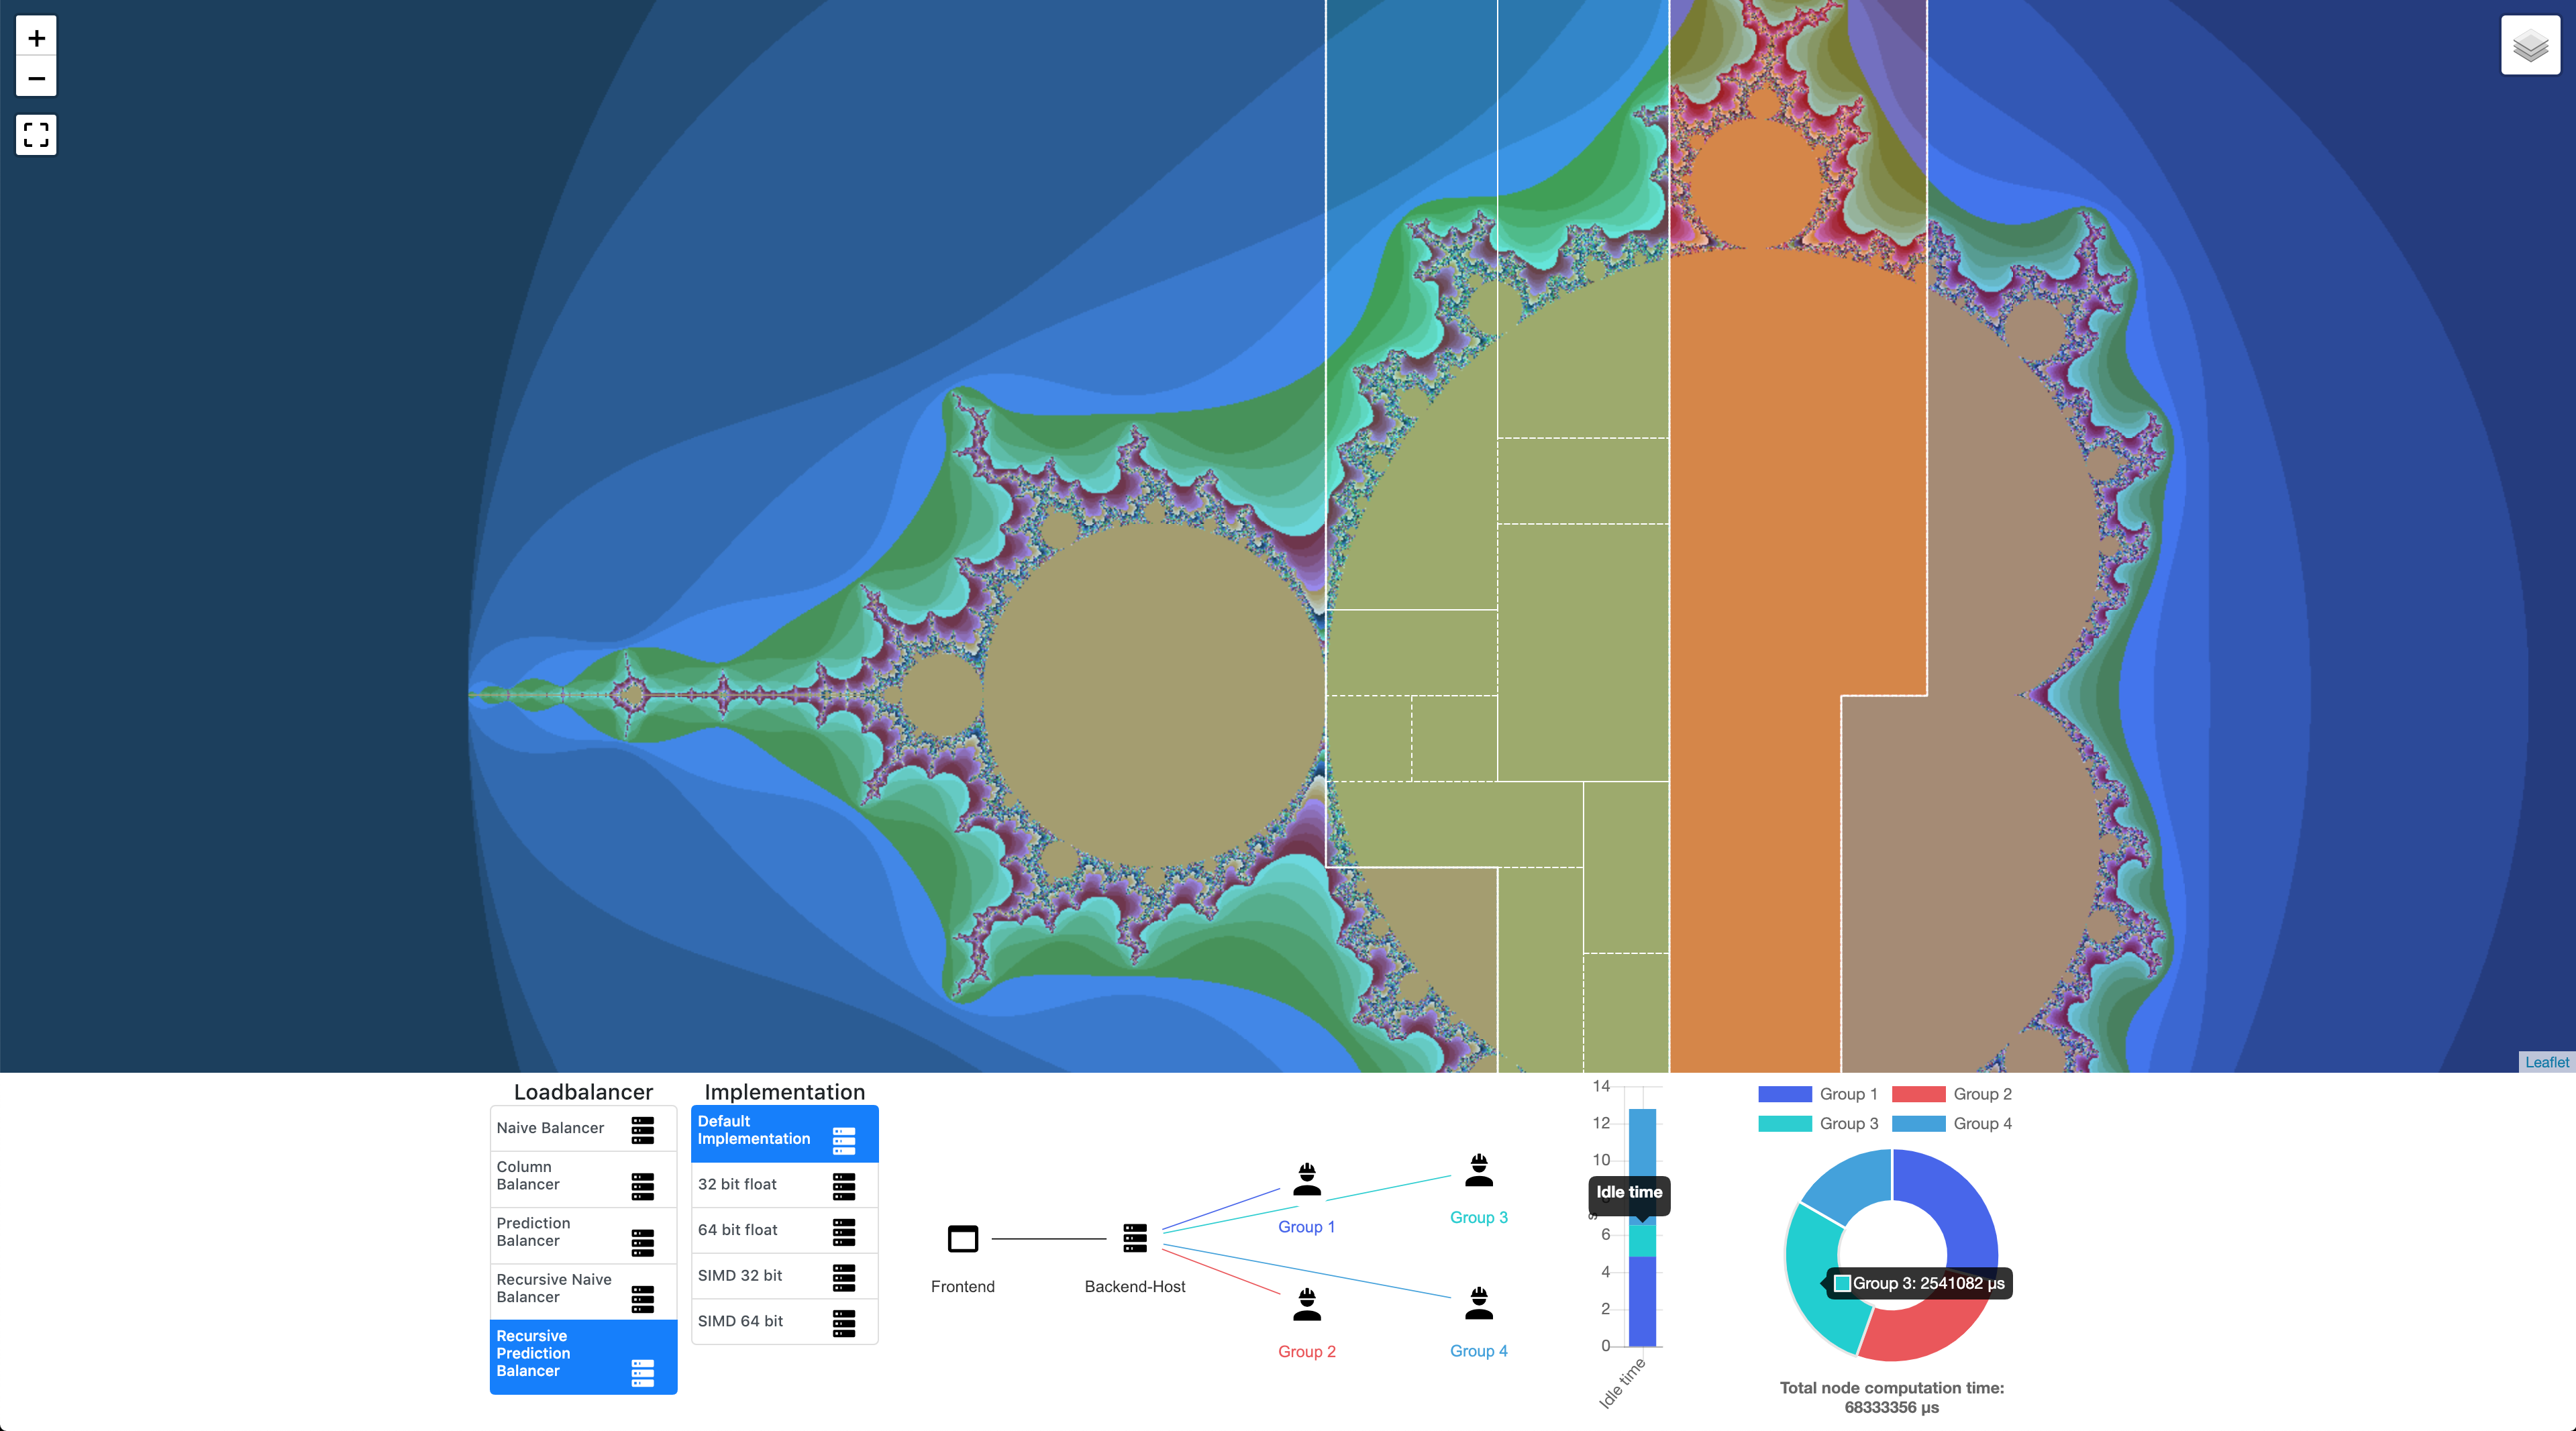
\includegraphics[width=\linewidth]{img/Implementierung/UI-Screenshot}
	\caption{Benutzeroberfläche der Mandelbrot Anwendung}
	\label{fig:ui-screenshot}
\end{figure}

\subsubsection{Kommunikation mit dem Backend}\label{sec:fontend_communication}

Zur Kommunikation mit dem Backend wird im Frontend ein Objekt der Klasse \verb|WebSocketClient| erzeugt.
Alle zur Verbindung mit dem Backend verwendeten Codestücke liegen dabei in dem Ordner \verb|src/connection/|.

Die dort definierte Klasse \verb|WebSocketClient| abstrahiert von dem JavaScript-nativen Websocketinterface \verb|WebSocket|\footnote{\url{https://developer.mozilla.org/en-US/docs/Web/API/WebSocket}}.
Bei der Initialisierung baut das erzeugte Objekt eine Verbindung zu der lokalen Adresse \url{ws://localhost:9002} auf\footnote{
	Faktisch wird eine Verbindung geöffnet, geschlossen und erneut geöffnet.
	Dies ist durch ein ungelöstes Problem beim Verbindungsaufbau bedingt, das dafür sorgt, dass ein Verbindungsaufbau
	erst bei der zweiten erzeugten Websocketverbindung fehlerfrei gelingt.
}.
Dort muss das Backend bereit sein, eine Websocketverbindung anzunehmen.

Die Klasse \verb|WebSocketClient| bietet dabei folgende Methoden:
\begin{itemize}
	\item \verb|sendRequest(request)|

	      Diese Methode versendet das übergebene RegionRequest-Objekt codiert als \verb|JSON|\footnote{\url{https://www.json.org/}}-Objekt an das Backend.
	\item \verb|registerRegion(fun), registerRegionData(fun)|

	      An diese Methoden können Callbacks übergeben werden, die aufgerufen werden, wenn das Frontend über die Websocketverbindung
	      respektive ein \texttt{Region}-Objekt oder ein \texttt{RegionData}-Objekt empfängt.
	      Diese sind die Aufteilung einer angefragten Region (siehe \autoref{src:region.json})
	      oder die berechneten Iterationswerte einer Region (siehe \autoref{src:regionData.json}).

	      Die übergebenen Callbacks erhalten als Parameter respektive die vorgruppierte Aufteilung als ein Array von Workergruppen (\texttt{RegionGroup})
	      oder das \verb|JSON|-dekodierte \verb|RegionData|-Objekt.

\end{itemize}
Zudem wird hierbei bereits eine Filterung der eingehenden Regionsdaten vorgenommen.
Bei Empfang einer Regionsaufteilung, wird diese zwischengespeichert.
Jedes empfangene Regionsdatenobjekt wird dann bei Empfang daraufhin überprüft,
ob der darin dargestellte Ausschnitt einer Regionsaufteilung entspricht (dazu wird das \verb|region|-Attribut verglichen)
und das dargestellte Fraktal der zuletzt übergebenen Auswahl entspricht.
Diese Filtrierung ist notwendig, da Worker Regionsdaten auch \enquote{verspätet} absenden können,
falls bei dem zuvorgehenden Bereich nicht gewartet wurde bis die Berechnungen aller Worker entgegengenommen wurden.
Die Definitionen der zugehörigen Objekt-Interfaces finden sich in den Dateien \verb|RegionGroup.ts| und \verb|ExchangeTypes.ts| finden.

Anfragen an das Backend werden dabei mit der folgenden Funktion in \verb|RegionRequest.ts| erstellt:
\begin{itemize}
	\item \verb|request(map, balancer, implementation)|:

	      Diese extrahiert aus der übergebenen Sicht auf die Mandelbrotmenge, die in der Leaflet-Karte gespeichert ist,
	      die Parameter zum Anfragen einer Region.
	      Dazu werden mithilfe des aktuellen Zooms der linke obere und rechte untere Punkt des Sichtbereiches
	      in dem Leaflet-internen Koordinatensystem auf entsprechende Punkte in der komplexen Ebene projeziert.
	      Da zum Erzeugen des passenden Objektes auch der gewünschte Lastbalancierer und der Fraktaltyp notwendig sind,
	      werden diese als weitere Parameter übergeben.

	      Die Funktion gibt direkt ein Objekt zurück, dass das Interface \verb|RegionRequest| erfüllt.
\end{itemize}

\subsubsection{Darstellung der Regionsdaten} % tileDisplay/

Die für die Darstellung der Mandelbrotmenge verwendete Bibliothek (leaflet) hat die Einschränkung, dass
nur Quadrate einer vordefinierten Größe (\verb|Tiles|) angezeigt werden können. Ebenfalls verwendet diese ein
eigenes Koordinatensystem, unter welchem jede angezeigte Tile eindeutig mit dem Tripel \( (x, y, zoom) \)
identifiziert wird. Somit ist eine Übersetzung zwischen den Daten des Backends und den von leaflet erwarteten nötig.

\paragraph{MatrixView.ts, RegionOfInterest.ts}\label{par:matrixView}
Die Klasse \verb|MatrixView.ts| implementiert die Umsetzung einer vom Backend versendeten Region zu
den von leaflet erwarteten Tiles.
\begin{itemize}
	\item \verb|registerTile(point, draw)|

	      Alle sichtbaren Tiles registrieren sich mit dem Callback \verb|draw|,
	      welcher ausgeführt wird, sobald die anzuzeigenden Daten für die
	      entsprechende Tile verfügbar sind. Diese Iterationswerte des Backends werden dabei der \verb|draw| Funktion als Parameter
	      in Form eines \verb|RegionOfInterest| Objekts übergeben.
\end{itemize}


Ein \verb|RegionOfInterest| Objekt implementiert wiederum die Übersetzung von lokalen \( (x,y) \) Pixel-Werten
einer Tile zu Indizes in das vom Backend gesendete Array an Regionsdaten (siehe \autoref{src:regionData.json}).
\begin{itemize}
	\item \verb|get(x, y)|

	      Gibt, für einen Tile \( (x,y) \) Pixel-Wert die benötigte Iterationsanzahl zurück.
	      %   (siehe \autoref{src:RegionOfInterest.ts}).
	      %   \begin{figure}[h!]
	      %       \lstinputlisting[caption={Umsetzung von Pixel-Werten der Tiles zu Indizes in Regionsdaten}, label={src:RegionOfInterest.ts}, language=TypeScript, firstline=41, lastline=48, firstnumber=41]{../../frontend/src/tileDisplay/RegionOfInterest.ts}
	      %   \end{figure}
\end{itemize}


\paragraph{TileDisplay.tsx}
Die Klasse \verb|TileDisplay.tsx| verwendet die leaflet Bibliothek direkt, um die Regionsdaten darzustellen.
Dabei wird dieser die WebSocket Verbindung in Form eines \verb|WebSocketClient|, sowie der vom Nutzer gewählte Balancer,
die Implementierung und Gruppierung durch \verb|Observable| Klassen (siehe \autoref{par:observables}) übergeben. Ebenfalls wird der anzuzeigende Ausschnitt der
Mandelbrotmenge übergeben.

Da das Backend die berechneten Teilbereiche der Mandelbrotmenge als Regionen zurück gibt, dessen Höhe und Breite
Vielfache der leaflet Tile-Größe sind, wird eine Region dem Benutzer durch mehrere Tiles dargestellt.
Dieses Verhältnis wird in \autoref{fig:leafletTiles} dargestellt.

\begin{figure}
	\centering
	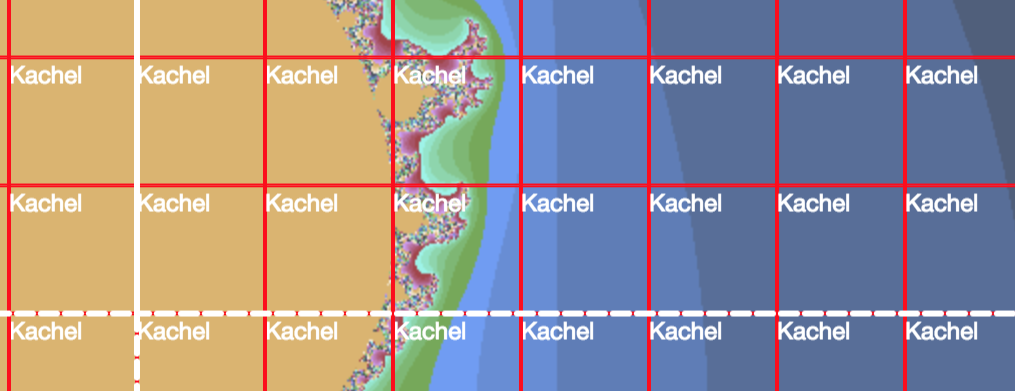
\includegraphics[width=0.5\linewidth]{img/Implementierung/leafletTiles}
	\caption{Relation von Backend Regionen zu leaflet Tiles.
		Dabei ist beispielhaft eine Region des Backends
		weiß eingezeichnet, alle leaflet Tiles sind rot umrandet angegeben.
	}\label{fig:leafletTiles}
\end{figure}

Zudem ist die Darstellung der Iterationswerte, sowie Regionsaufteilung durch unterschiedlichen Ebenen innerhalb der
leaflet Bibliothek realisiert:

\begin{itemize}
	\item \verb|MandelbrotLayer| in \verb|TileDisplay.tsx|

	      In dieser eigenen Ebene der leaflet karte werden die Tiles dargestellt.
	      Dieser erstellt für den sichtbaren Bereich\footnote{
		      Da die Fenstergröße des sichtbaren Bereichs keien Vielfaches der Tilegröße sein muss,
		      können Tiles erzeugt werden, welche teilweise außerhalb des sichtbaren Beriechs liegen}
	      alle benötigten Tiles. Für jede der Tiles wird ein \verb|HTML5 canvas|\footnote{\url{https://developer.mozilla.org/kab/docs/Web/API/Canvas_API}} Objekt erstellt, welches es
	      ermöglicht, für jeden Pixel einen \( (r,g,b) \) Farbwert zu definierten und anzuzeigen. Wobei die Farbwerte aus den berechneten
	      Iterationswerten des Backends mit einem Shader (siehe \autoref{par:shader}) ermittelt werden. Die Iterationswerte können wiederum
	      mit einem \verb|MatrixView| Objekt aus den Regionsdaten des Backends gelesen werden.

	\item \verb|WorkerLayer| in \verb|WorkerLayer.ts|\label{par:workerLayer}

	      Diese Klasse visualisiert die Regionsaufteilung des Lastbalancierers als Overlay, welche über den Iterationswerten
	      dem Benutzer angezeigt wird.
	      Dafür wir eine in leaflet bestehende \verb|GeoJSON| API verwendet, mit welcher es möglich
	      ist, beliebige Polygone auf den bestehenden Kartendaten anzuzeigen. Die Knoten dieser Polygone werden dabei jede \verb|RegionGroup|
	      mit Hilfe der Funktionen aus \verb|Project| von Koordinaten der komplexen Ebene, welche im Backend verwendet werden, zu
	      leaflet Koordinaten umgerechnet.

	      \begin{figure}
		      \centering
		      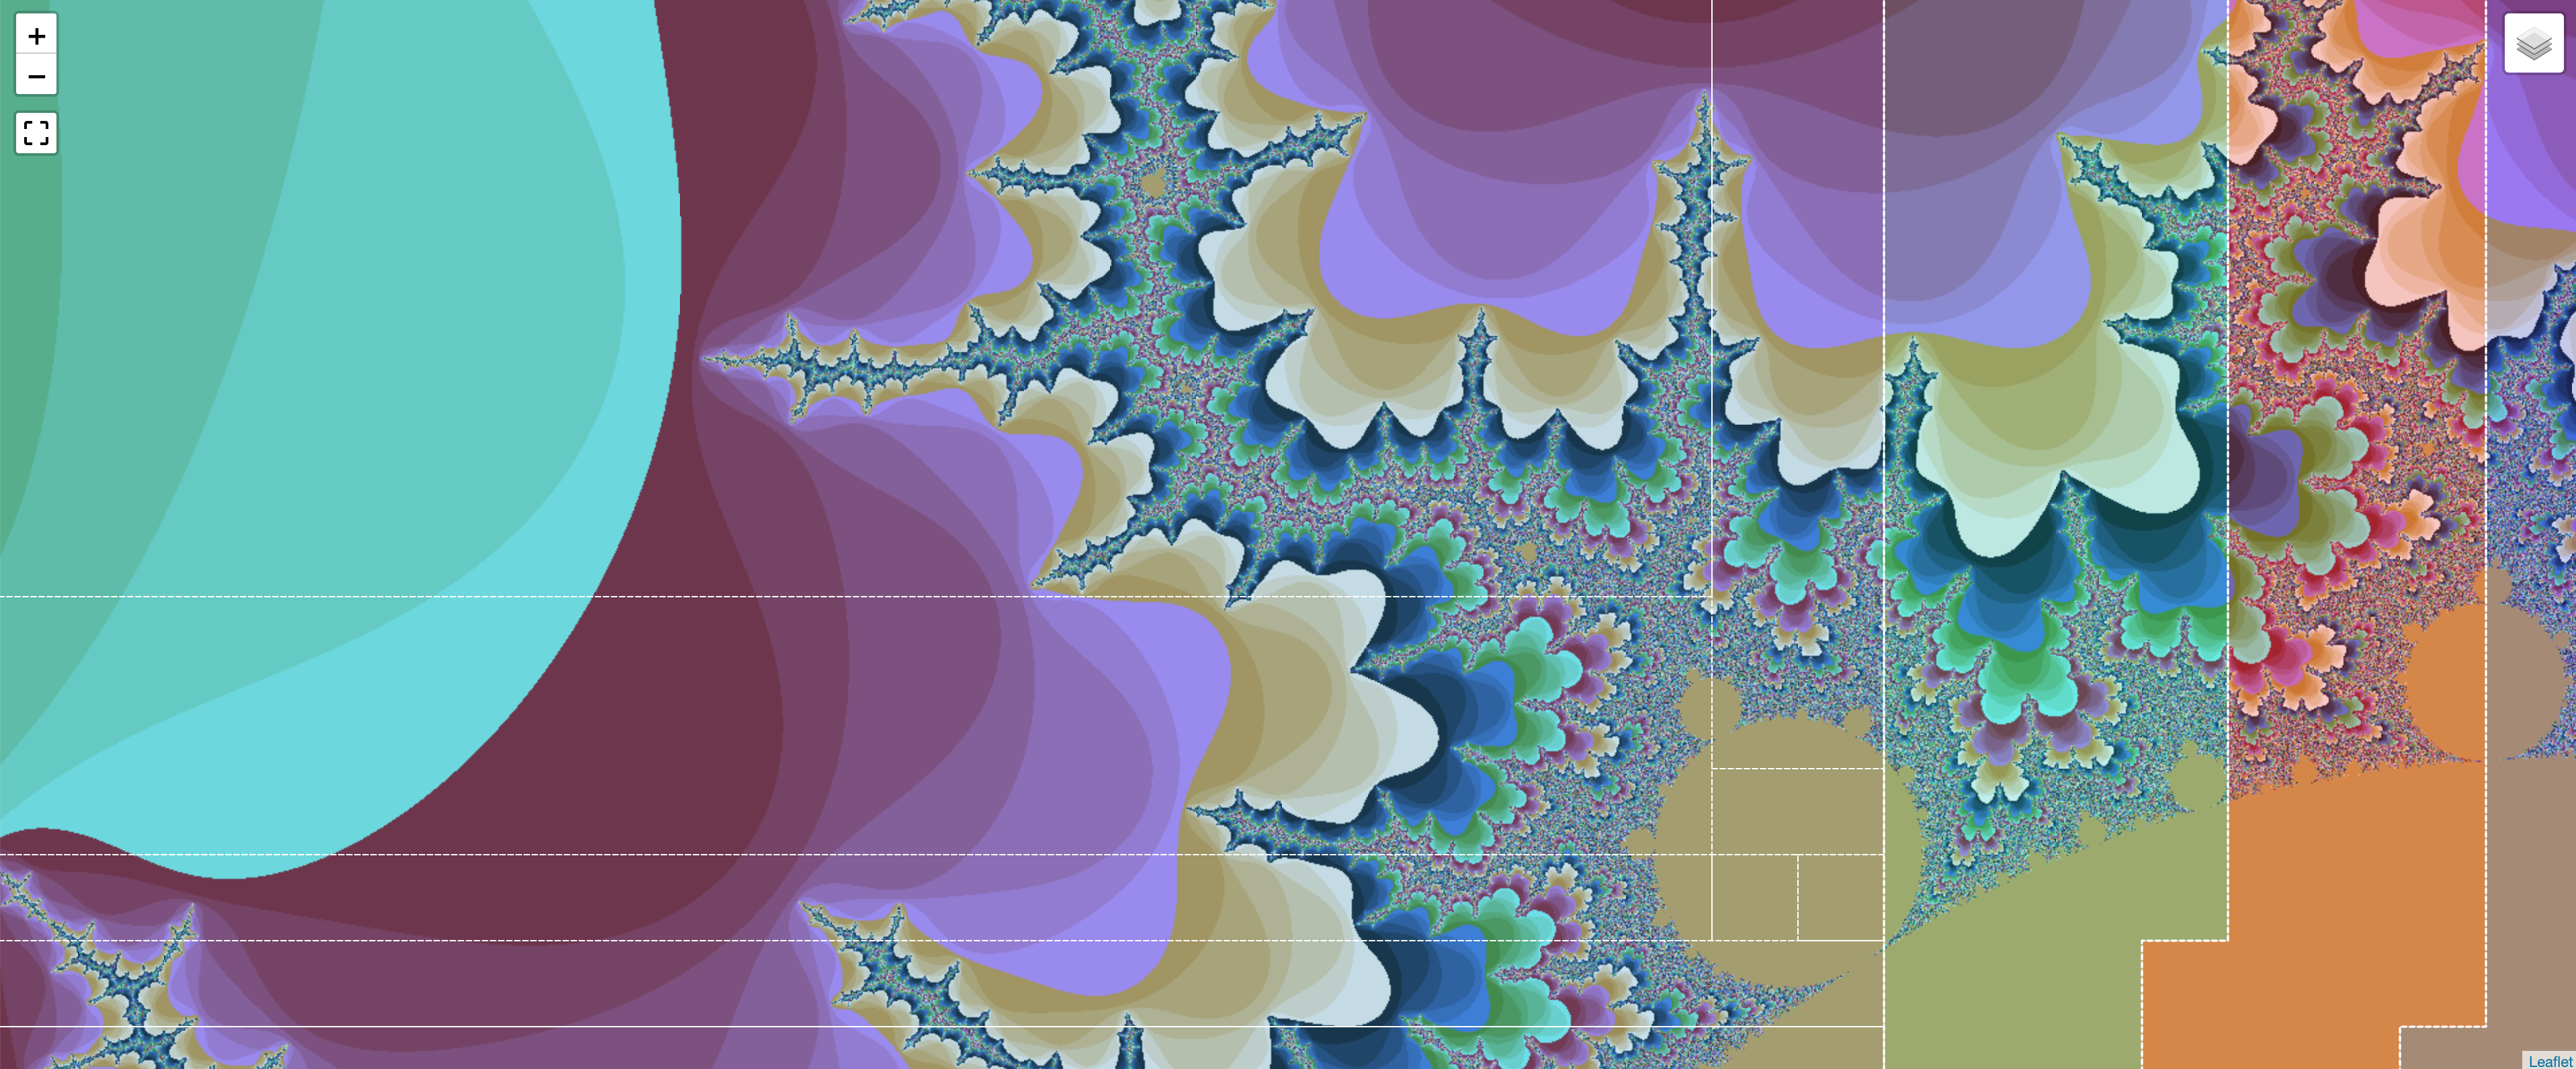
\includegraphics[width=.85\linewidth]{img/Implementierung/regionGrouping}
		      \caption{WorkerLayer für eine Gruppierung der Aufteilung des Recursive PredictionBalancers mit 37 Workern}
		      \label{fig:regionGrouping}
	      \end{figure}

	      Da es wie in \autoref{par:regionGroup} beschrieben zu einer Gruppierung kommt, falls die Anzahl der Worker im Backend zu
	      groß ist, werden ebenfalls alle Untergruppen einer Gruppe angezeigt (siehe \autoref{fig:regionGrouping}), falls der Benutzer mit der Maus über eine der
	      dargestellen Gruppierungen geht.
	\item \verb|DebugLayer| in \verb|TileDisplay.tsx|

	      Diese Ebene gibt Informationen zur Aufteilung der angezeigten leaflet Tiles und den Projektionen von
	      leaflet Koordinaten zu komplexen Koordinaten.
\end{itemize}


\paragraph{Shader.ts}\label{par:shader}
Berechnet für einen Iterationswert der Mandelbrotmenge ein Tripel \( (r,g,b) \) von Farbwerten.
Implementiert ist eine simple Funktion, welche den Iterationswert für jeden Farbkanal mit einer Konstante multipliziert
und auf den zulässigen ganzzahligen Wertebereich \( [0,255] \) abbildet (siehe \autoref{src:Shader.ts}).

\begin{figure}[h!]
	\lstinputlisting[caption={Berechnung der \( (r,g,b) \) Farbwerte}, label={src:Shader.ts}, language=TypeScript, firstline=2, lastline=7, firstnumber=2]{../../frontend/src/tileDisplay/Shader.ts}
\end{figure}

\paragraph{Project.ts}
Da die leaflet Bibliothek Tiles verwendet, um die Regionen des Backends anzuzeigen, liegen diese in
einem neuen Koordinatensystem, welches jeder Tile auf für eine Zoomstufe ein Triple \( (tileX, tileY, zoom) \) zuordnet.
Weiterhin besitzt leaflet ein internes Koordinatensystem (CRS\footnote{\url{https://en.wikipedia.org/wiki/Spatial_reference_system}}),
welches jeden Punkt auf der Karte durch das Paar \( (latitude, longitude) \) identifiziert.
\verb|Projekt.ts| enthält Funktionen, um zwischen diesen 3 Koordinatensystemen
(Tile-Koordinaten, leaflet-Koordinaten und Koordinaten der komplexen Ebene) zu konvertieren.

% TODO:
\paragraph{Regionsgruppierung (RegionGroup.ts)}\label{par:regionGroup}

\subsubsection{Visualisierung der Architektur des Backends}

Die Struktur der Parallelisierung wird in einem Netzwerkgraphen unter dem Fraktal dargestellt.
Mithilfe der Bibliothek \verb|visjs|\footnote{\url{http://visjs.org/}} wird hierzu ein
Graph (siehe \autoref{fig:networkView}) mit 3 Ebenen erzeugt:

Auf der linken Seite befindet sich ein Knoten in Form eines Programmfensters, der das Browserfrontend darstellt.
In der Mitte wird ein Knoten für den Backend-Host mit Serverrack als Symbol dargestellt, der mit dem Frontendknoten verbunden ist.
Auf der rechten Seite befindet sich schließlich zwischen 2 und 4 Knoten, die jeweils eine Gruppe an Arbeitern
darstellen. Das Symbol hierfür ist ein Oberkörper mit Arbeitshelm.
Sie sind wiederum direkt mit dem Host verbunden.

Der Code für diese Darstellung findet sich in \verb|components/NetworkView.tsx|.
Dort wird ein Baumgraph von links nach rechts mit manueller Ebenenverteilung als Grundstruktur für die Darstellung des Graphen definiert.
Daher wird das Frontend auf der höchsten Ebene und der Backend-Host auf der Ebene darunter spezifiziert.
Die Arbeiter werden auf Basis der erhaltenen Regionsaufteilung erzeugt und jeweils zu zweit nacheinander
auf Ebenen verteilt.
Diese Aufteilung wird nach Erhalt jeder Regionsaufteilung vorgenommen und der Graph neu aufgebaut,
sowie die Größe der Leinwand an die Anzahl an Knoten angepasst.

\begin{figure}
	\centering
	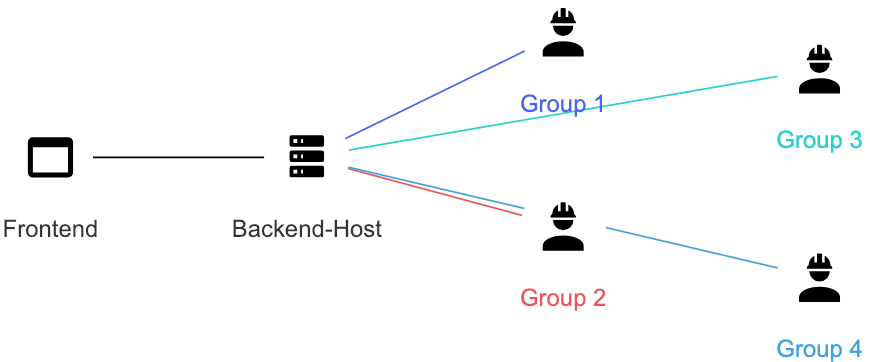
\includegraphics[width=0.5\linewidth]{img/Implementierung/NetworkView}
	\caption{Darstellung der Architektur der Anwendung als Graph
	}\label{fig:networkView}
\end{figure}

\subsubsection{Visualisierung der Rechenzeiten} % components/

Die zeitbezüglichen Komponenten der Visualisierung werden mithilfe der Charts
der Bibliothek \verb|chartjs|\footnote{\url{http://www.chartjs.org/}} dargestellt.
\begin{figure}
	\centering
	\begin{minipage}{.5\textwidth}
		\centering
		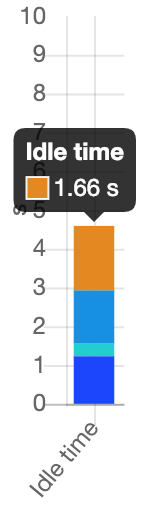
\includegraphics[height=.5\linewidth]{img/Implementierung/IdleTime}
		\caption{Idle Time für 5 Gruppen}
		\label{fig:idleTime}
	\end{minipage}%
	\begin{minipage}{.5\textwidth}
		\centering
		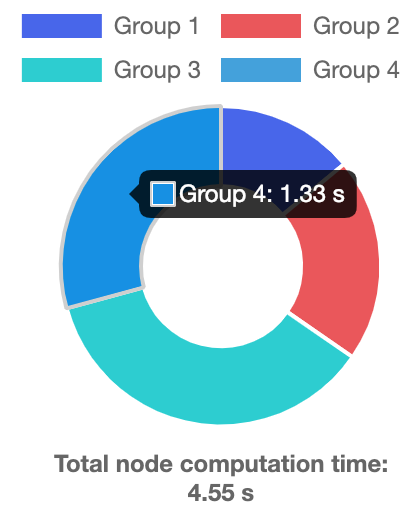
\includegraphics[height=.5\linewidth]{img/Implementierung/ComputationTime}
		\caption{Computation time für 4 Gruppen}
		\label{fig:computationTime}
	\end{minipage}
\end{figure}

\paragraph{Idle Time}

Für die kritische Information der verschwendeten Zeit wird ein Balkengraph verwendet.
Dieser besitzt einen Balken, der die Differenz zwischen der Rechenzeit aller Knoten und dem am längsten rechnenden Knoten
aufsummiert und nach Gruppe sortiert darstellt (siehe \autoref{fig:idleTime}).

Die Darstellung wird bei Empfang einer Regionsaufteilung (mithilfe \verb|registerRegion| in \verb|WebSocketClient|)
initialisiert indem die Anzahl an Knoten und die Gruppen gespeichert, die Rechenzeit der Knoten auf \( 0 \) gesetzt und
alle Knoten als aktiv markiert werden.
Da die tatsächliche Rechenzeit erst am Ende der Berechnung mit den Regionsdaten selbst verfügbar ist,
wird mithilfe eines Intervalls die Rechenzeit live abgeschätzt, indem sie alle \( 50ms \) um
\( 50ms \) hochgezählt wird, falls die Regionsdaten des Knotens noch nicht empfangen wurden.

Da die Charts nicht zur Animation von Übergängen fähig sind, wird das Objekt mit jedem Update neu gerendert.
Bei Empfang von Regionsdaten (hierzu wird die erwähnte Methode \verb|registerRegionData| verwendet)
wird die tatsächlich gemessene Rechenzeit eingetragen und der Rechenknoten als inaktiv gekennzeichnet.
Der Intervall wird gestoppt, sobald alle Arbeiterknoten die Berechnung abgeschlossen haben.

\paragraph{ComputationTime}

Zur Darstellung des relativen Verhältnisses der Rechenzeiten wird in einem Kuchengraph
die absolute Rechenzeit der Gruppen dargestellt (siehe \autoref{fig:computationTime}).

\subsubsection{MISC} % misc/

\paragraph{Observable.ts}\label{par:observables}